\section{Antecedentes}

FHIR (Fast Health Interoperability Resources) es un estándar para intercambiar información del cuidado de la salud electrónicamente \cite{FHIRClinician}. FHIR ofrece un fuerte enfoque en la implementabilidad en una amplia variedad de arquitecturas y escenarios \cite{FHIRExecutive}. La versión actual de FHIR se publica como un estándar para uso experimental \cite{FHIR}.

OpenEHR es un enfoque de plataforma para el desarrollo de soluciones de tecnología de la información para el cuidado de la salud. OpenEHR provee un conjunto de estándares para modelos de información clínica, extractos de EHR, datos demográficos, tipos de datos y varios tipos de interfaces de servicio \cite{openEHRWhitePaper}.

\subsection{FHIR}

FHIR define recursos para representar conceptos administrativos tales como paciente, proveedor, organización y dispositivo, así como conceptos clínicos que cubren problemas, medicamentos, diagnósticos, planes de atención y más \cite{FHIRResourceList}.

Los recursos tienen en común las siguientes características \cite{FHIRDeveloper}:
\begin{itemize}
  \item una URL que identifica el recurso;
  \item una metainformación común;
  \item un texto legible por el ser humano para la seguridad clínica;
  \item un conjunto definido de elementos de datos diferente para cada recurso;
  \item un marco para extender y adaptar los recursos existentes.
\end{itemize}

Los recursos se describen usando recursos StructureDefinition \cite{FHIRStructureDefinition}. Estos recursos StructureDefinition definen un conjunto de elementos de datos. Cada elemento incluye una ruta, una cardinalidad y un tipo de dato \cite{FHIRElementDefinition}.

La ruta del elemento de dato es la propiedad más importante de la definición del elemento. Esta ruta localiza el elemento en una jerarquía definida dentro del recurso \cite{FHIRElementDefinition}.

El tipo de dato del elemento de dato puede ser primitivo o complejo \cite{FHIRDataTypes}. La diferencia entre ambos tipos de datos es que el primitivo permite un solo valor para el elemento,  mientras que el complejo puede tener elementos hijos. Cada tipo de dato primitivo es una 3-tupla, que consiste en a) un dominio de valores, que incluye la definición del tipo de dato, b) una representación XML y c) una representación JSON. Dentro de los tipos de datos complejos se encuentran: los de propósito general, los tipos para metadatos y los de propósito especial.

Cada elemento de dato puede ser extendido o restringido \cite{FHIRProfiling}. El elemento de dato se extiende para representar información adicional que no forma parte de la definición del recurso\cite{FHIRExtensibility}. Cada recurso solo incluye elementos de datos si la mayoría de las implementaciones usarán esos elementos de datos en particular \cite{FHIRArchitecture}. El elemento de dato se restringe cambiando su cardinalidad.

Los recursos soportan la vinculación a terminología clínica, lo cual contribuye al uso de FHIR para lograr la interoperabilidad semántica \cite{FHIRArchitecture}.

Aparte de las definiciones de los recursos, FHIR define un conjunto de interfaces por las cuales los sistemas comparten los recursos. Los mecanismos de intercambio soportados son los siguientes \cite{FHIRClinician}:
\begin{itemize}
  \item a través de una interfaz REST;
  \item mediante el intercambio de documentos;
  \item vía el envío y recepción de mensajes;
  \item la exposición e invocación de servicios.
\end{itemize}


\subsection{openEHR}

El enfoque de openEHR es un riguroso modelado del conocimiento, y se basa en el principio básico de separación de los dominios de concepto y los dominios de información en los sistemas de información. Los dominios de concepto son modelados usando los arquetipos y expresados en el Lenguaje de Definición de Arquetipos (ADL). Estos conceptos son profundizados a continuación.

\subsubsection{Modelado en openEHR}

El enfoque de openEHR para el modelado es multinivel. Los modelos son desarrollados y mantenidos por expertos de dominio en su propio nivel \cite{openEHRArchitecture}.

El primer nivel se basa en el modelo de referencia. El modelo de referencia corresponde al modelo de información estable, por ejemplo, tipos de datos o estructuras de datos. Todos los datos EHR en cualquier sistema openEHR obedecen el modelo de referencia. Solo este primer nivel es implementado en software \cite{openEHRArchitecture}.

El siguiente nivel consiste en los arquetipos. Los arquetipos corresponden a los contenidos del dominio, por ejemplo, medidas de la presión sanguínea o resultado de la prueba para diabetes. Estos arquetipos son modelados por profesionales clínicos o expertos en informática de la salud sin ningún conocimiento tecnológico de los sistemas finales. Los arquetipos son almacenados en sus propios repositorios.

Las plantillas constituyen el siguiente nivel. Estas plantillas especifican grupos de arquetipos que se usan para un propósito particular, y a menudo corresponden a formularios de pantalla \cite{openEHRArchitecture}.

En el último nivel se encuentran los artefactos generados a partir de las plantillas. Estos artefactos pueden ser interfaces de programas, XSDs, componentes de interfaces de usuarios \cite{openEHR}.

La Figura \ref{fig:openeEHR_ecosystem} ilustra el modelado multinivel.

\begin{figure}[h]
  \centering
  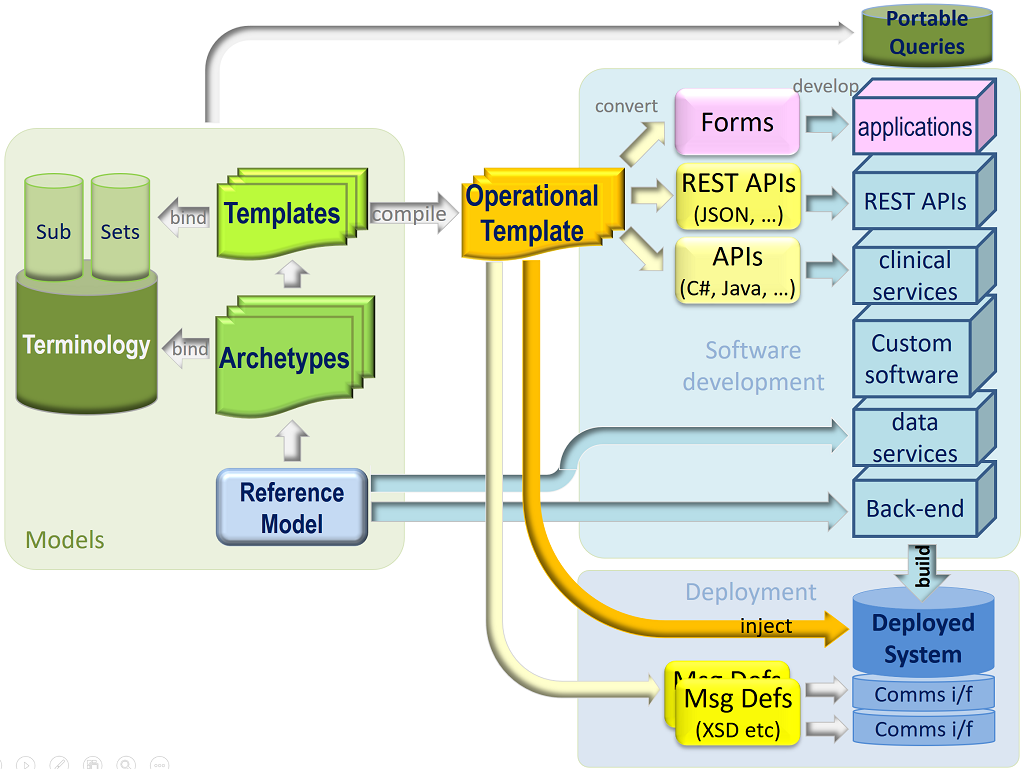
\includegraphics[scale=0.6]{./images/openehr_dev_ecosystem}
  \caption{Enfoque openEHR}
  \label{fig:openeEHR_ecosystem}
\end{figure}


\subsubsection{Arquetipos}

Cada arquetipo es un conjunto de restricciones en el modelo de referencia, definiendo un contenido de dominio \cite{openEHRArchitecture}. Las restricciones definen configuraciones de instancias del modelo de referencia consideradas conformes al arquetipo. Por ejemplo, ciertas configuraciones de las clases PARTY, ADDRESS, CLUSTER y ELEMENT pueden definirse por un arquetipo Person como estructuras permitidas para personas con identidad, contactos y direcciones \cite{openEHRAOM}.

Los arquetipos pueden tener relaciones de especialización y/o composición. Los arquetipos especializados son creados restringiendo aún más las restricciones existentes de otros arquetipos. Los arquetipos compuestos son definidos a partir de otros arquetipos \cite{openEHRArchitecture}.

OpenEHR incluye un mecanismo de rutas. Estas rutas pueden usarse para referenciar a cualquier dato dentro de un arquetipo \cite{openEHRArchitecture}.

Los arquetipos proveen una forma de definir el significado de los datos, y de conectar los datos a terminologías conocidas como SNOMED CT, LOINC, ICPC, ICDx y muchas otras terminologías y vocabularios usados en salud \cite{openEHRArchitecture}.


\subsubsection{Lenguaje de Definición de Arquetipo}

Los arquetipos son expresados en el Lenguaje de Definición de Arquetipo \cite{openEHRADL} (ADL por sus siglas en inglés). ADL utiliza tres sintaxis: cADL (forma de restricción de ADL), ODIN (notación de instancia de datos de objeto) y una versión de lógica de predicado de primer orden (FOPL por sus siglas en inglés).

Las restricciones de cADL se escriben en un estilo estructurado en bloques, similar a los lenguajes de programación estructurados en bloques como C. Cada bloque se introduce mediante un identificador de un modelo de información de openEHR. Los identificadores alternan entre los nombres de tipo conocidos como bloques de objetos o nodos de objeto y los nombres de atributos de tipo conocidos como bloques de atributo o nodos de atributos. El uso de nodos de objeto permite la formación de rutas de arquetipo, que se pueden utilizar para hacer de forma inequívoca a nodos de objetos dentro del mismo arquetipo \cite{openEHRADL}.

La sintaxis de cADL se utiliza para expresar la definición de los arquetipos, mientras que la sintaxis de ODIN se usa para expresar datos que aparecen en las secciones de idioma, descripción, terminología y revisión histórica de un arquetipo.

Actualmente hay dos versiones principales existentes: `ADL 1.4', la versión original, y `ADL 2', una versión más moderna, que se está adoptando lentamente.



FHIR y openEHR comparten cierta similitud. Los recursos de FHIR y los arquetipos de openEHR definen patrones reutilizables para la descripción precisa de la información clínica \cite{Bosca15}. Sin embargo, los trabajos de colaboración entre las comunidades de FHIR y openEHR \cite{Collaboration} no consiguieron generar recursos y arquetipos con un contenido coincidente y clínicamente verificable. Una de las causas son los principios de diseño diferentes utilizados por ambas comunidades. Siendo la principal diferencia que los arquetipos esperan representar la mayoría del contenido clínico, mientras que los recursos solo contienen la información clínica utilizada más común.

El enfoque propuesto en este trabajo utiliza los recursos FHIR StructureDefinition para crear nuevos arquetipos openEHR. Estos nuevos arquetipos, expresados en ADL, facilitarán el intercambio de datos entre sistemas FHIR y sistemas openEHR. El intercambio se logra estableciendo mapeos entre las rutas de los elementos de los recursos y las rutas de los nodos de los arquetipos. Además, el enfoque propuesto hace uso de vinculaciones, conexiones entre modelos de información y terminologías, soportados por ambos estándares para conservar el significado de los datos intercambiados. 
